\chapter{TDT4295 - Computer Design Project}
\label{sec:intro}

The Computer Design Project is held at NTNU every fall.
It is a large, project-based subject in which students create a working computing platform, more or less from scratch.
This year saw high enough participation that two assignments were presented, and two groups formed around these.
This report details the work done and solution implemented by the vector graphics processor group.

\section{Assignment}

This years assignment focuses on graphics, exploring both of the traditional ways of representing and processing graphics; raster-based and vector-based.
Two distinct assignment texts were presented by the course staff, one focusing on raster-based graphics, the other on vector graphics.
The following is a verbatim copy of the vector graphics assignment text \cite{assignment-text}.

\subsection{Assignment Text - A Vector Graphics Processor}

Image generation using vector graphics as the core method is a powerful and scalable way of generating image data.
Vector graphics represents images at a higher abstraction level than single-pixels.
A vector graphics processor can make use of drawing instructions to produce images, which is a task well suited for hardware acceleration [3 // TODO: add references].
Parallelization with multiple cores and/or at the instruction level are architectural possibilities that can be exploited to design a specialized processor.
The task is to design and implement a processor for producing vector graphics.
Figure \ref{fig:vector-display-network-analyzer} illustrates a vector display which takes in vector drawing commands (instead of a stream of pixels) as input.

\begin{figure}[h!]
    \centering
    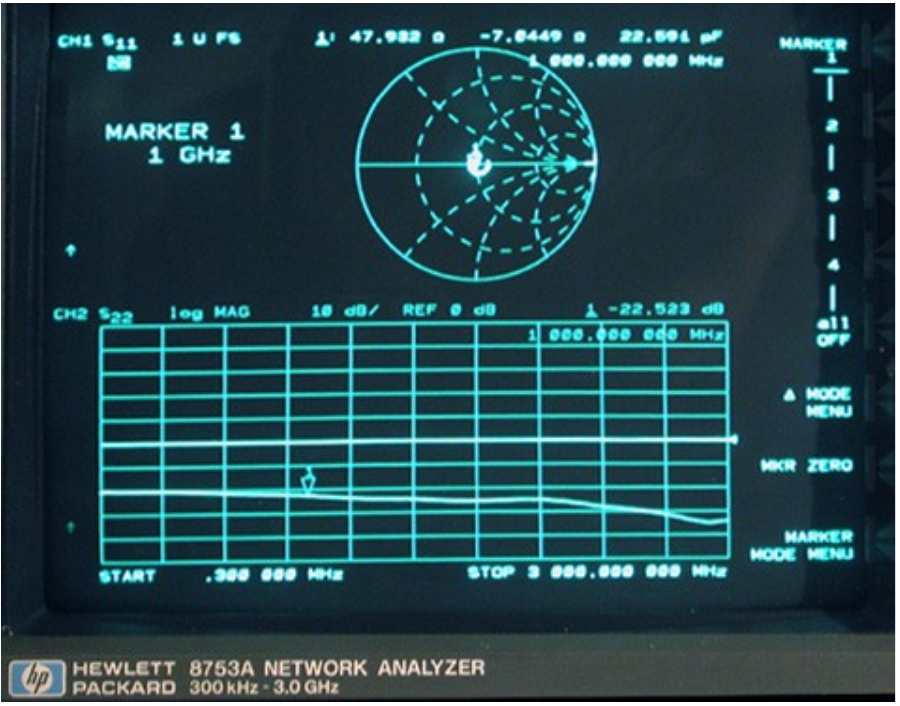
\includegraphics[width=0.8\linewidth]{images/network-analyzer-vector-graphics-display.png}
    \caption{A vector graphics display on a network analyzer\cite{assignment-text}.}
    \label{fig:vector-display-network-analyzer}
\end{figure}

\section{Vector Graphics - A Short Introduction}



\section{A Vector Graphics Computer Architecture}

The group chose to make a general purpose computer with support for producing vector graphics.
The computer would read instructions from memory, execute them on a processor core and render vector based scenes to different outputs.
Since most commonly available display devices expect raster based input, an oscilloscope was chosen as the primary output device, HDMI as a secondary.
This means that in addition to a processor core and memory interfaces, output preprocessors for both output modes would have to be implemented.
In the case of HDMI, a rasterizer, and for oscilloscope output, a serializer feeding data to DACs.

As a whole, the system should be assembled on a custom PCB, with the microcontroller serving as an I/O-unit while the main processor architecture and output-modules should be implemented on the FPGA.
The microcontroller would be tasked with loading a program into memory on boot, so that the processor has something to work with.

\section{Requirements}

// TODO: Add all requirements in list/table here

\section{About this report}

// TODO: Outline report contents.
